%\documentclass{standalone}
%\usepackage{pgfplots}
%\usepackage{bm}
%\usepackage{siunitx}
\pgfplotsset{compat=1.12}
\usetikzlibrary{arrows, decorations.pathmorphing, backgrounds, positioning,fit,petri}
\usetikzlibrary{calc}

\newcommand{\xdistl}{6cm}
\newcommand{\xdistr}{4cm}

\begin{document}

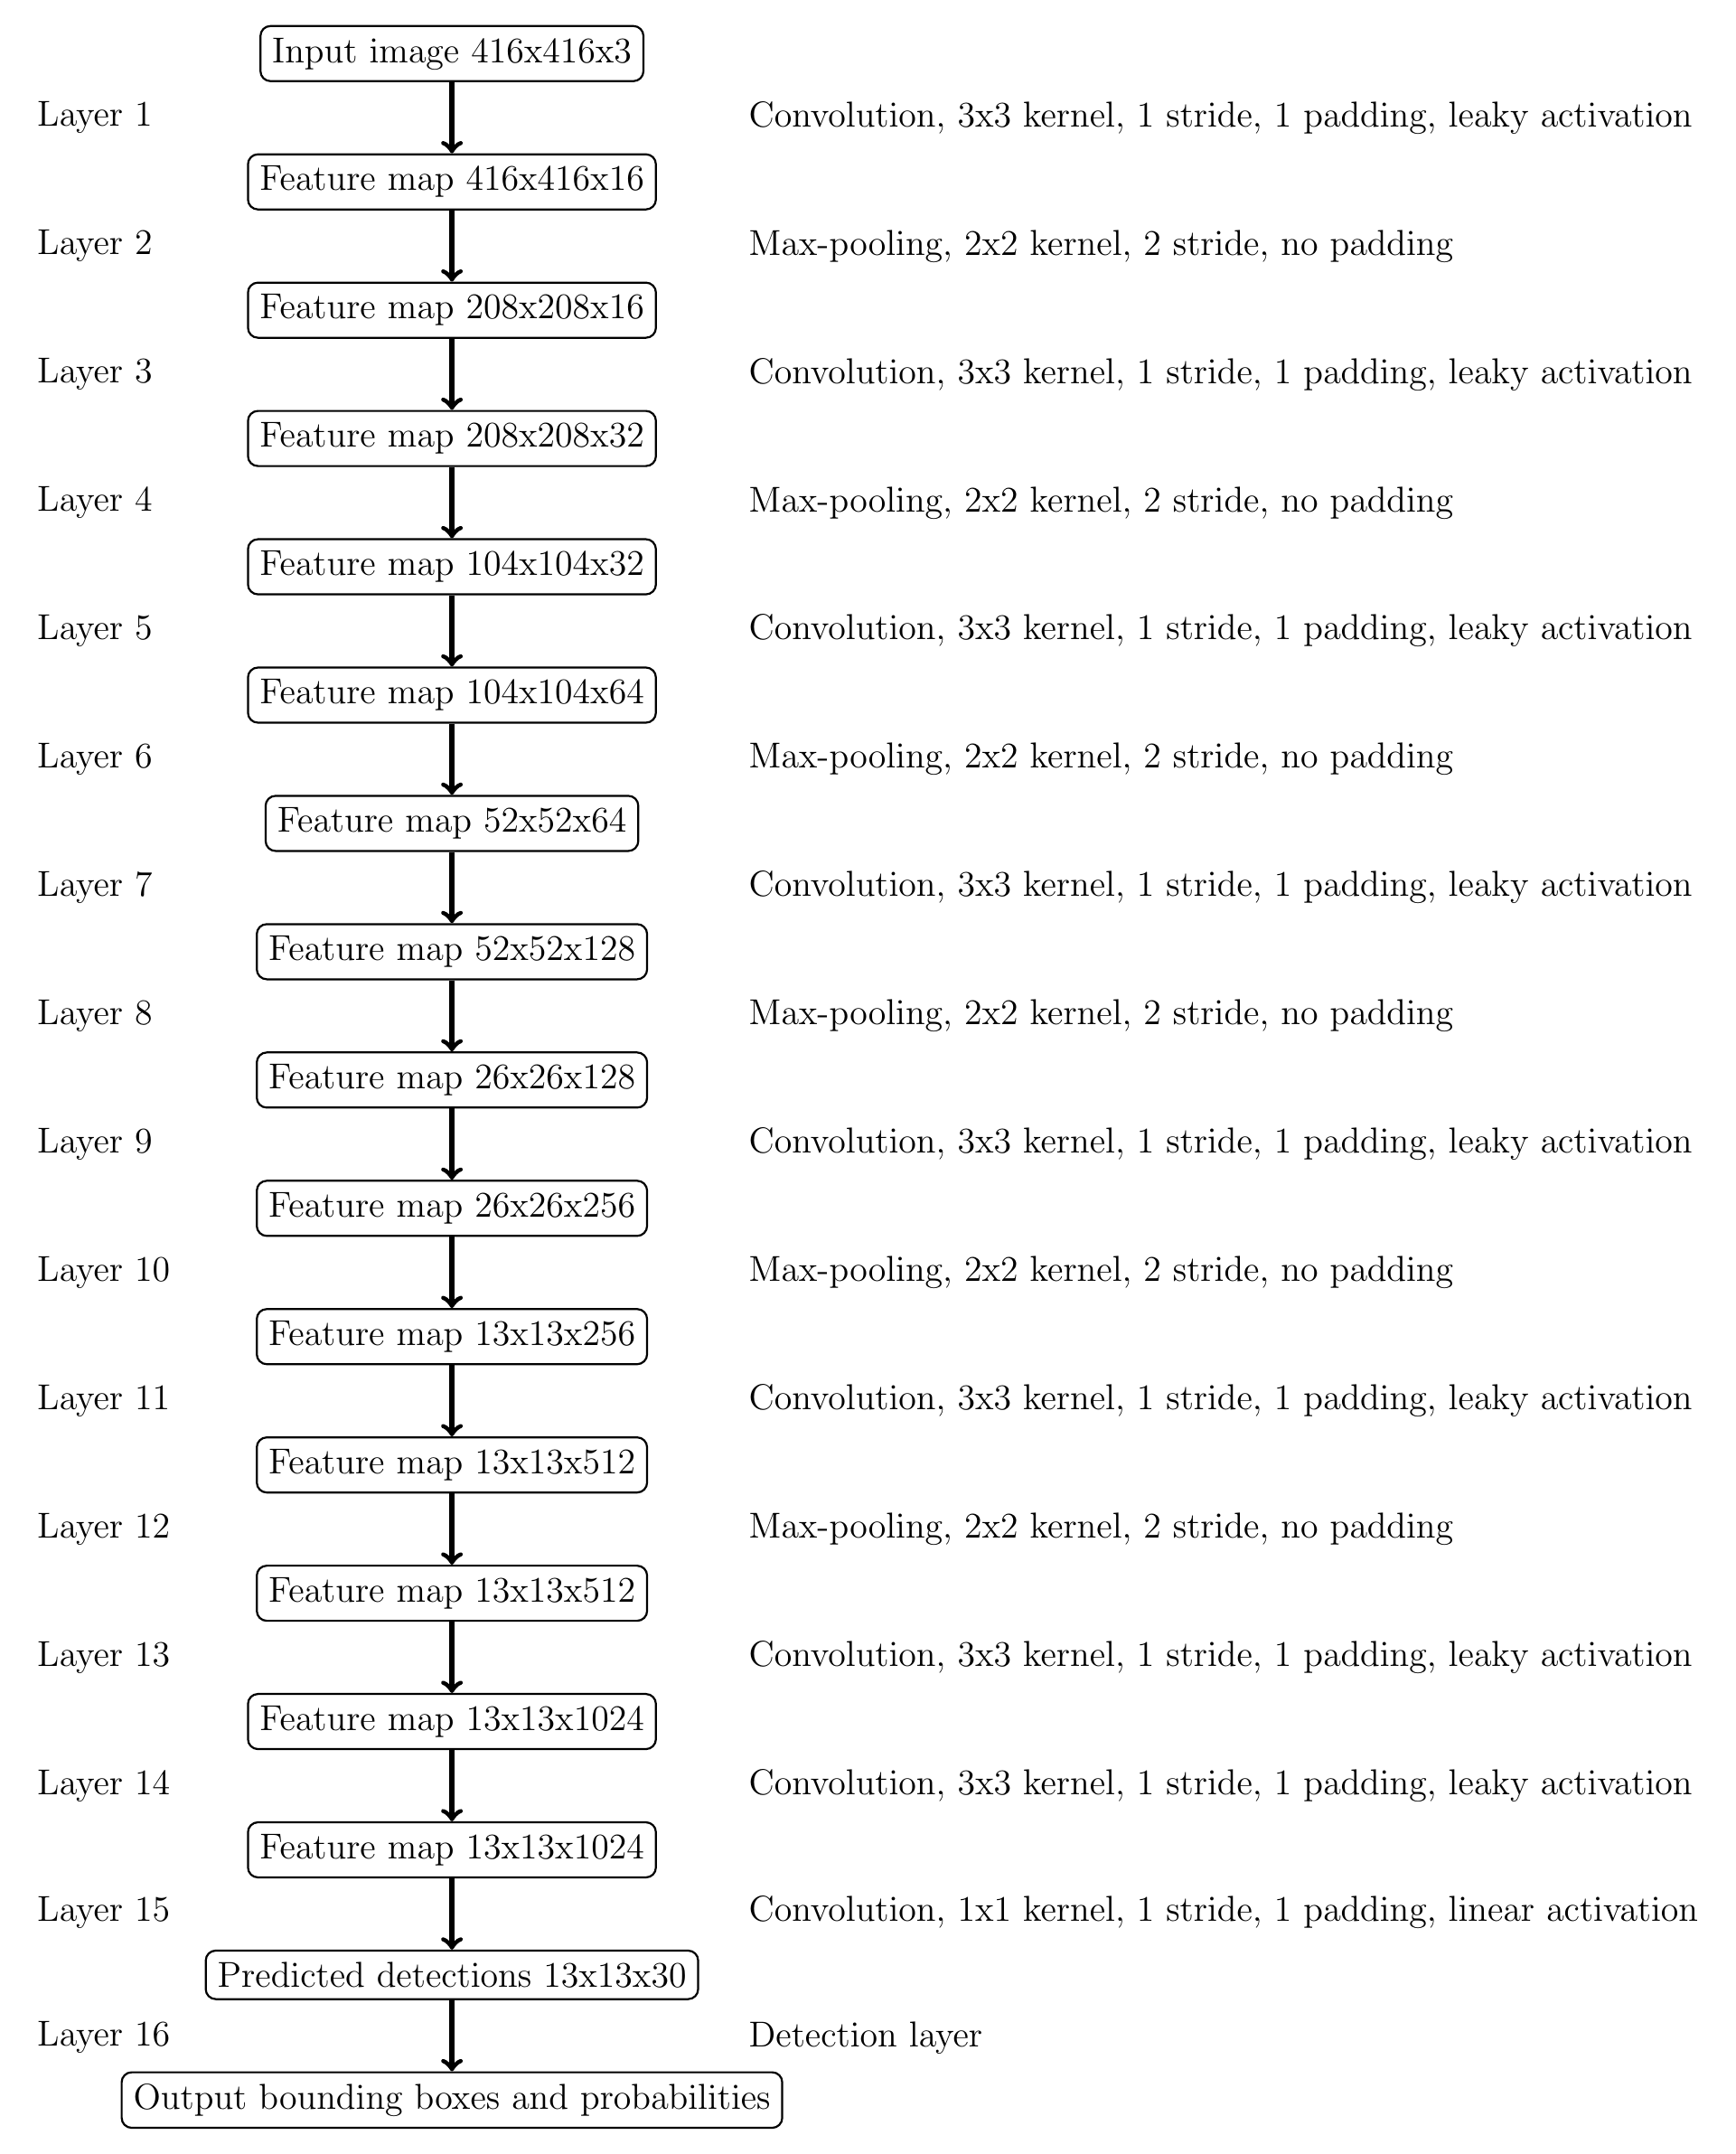
\begin{tikzpicture}
  \fontsize{15}{15}
  {
    \node[black, draw, thick, rounded corners] (f1) at (0, 0) {Input image 416x416x3};
    \node[black, draw, thick, rounded corners] (f2) [below=of f1] {Feature map 416x416x16};
    \node[black, draw, thick, rounded corners] (f3) [below=of f2] {Feature map 208x208x16};
    \node[black, draw, thick, rounded corners] (f4) [below=of f3] {Feature map 208x208x32};
    \node[black, draw, thick, rounded corners] (f5) [below=of f4] {Feature map 104x104x32};
    \node[black, draw, thick, rounded corners] (f6) [below=of f5] {Feature map 104x104x64};
    \node[black, draw, thick, rounded corners] (f7) [below=of f6] {Feature map 52x52x64};
    \node[black, draw, thick, rounded corners] (f8) [below=of f7] {Feature map 52x52x128};
    \node[black, draw, thick, rounded corners] (f9) [below=of f8] {Feature map 26x26x128};
    \node[black, draw, thick, rounded corners] (f10) [below=of f9] {Feature map 26x26x256};
    \node[black, draw, thick, rounded corners] (f11) [below=of f10] {Feature map 13x13x256};
    \node[black, draw, thick, rounded corners] (f12) [below=of f11] {Feature map 13x13x512};
    \node[black, draw, thick, rounded corners] (f13) [below=of f12] {Feature map 13x13x512};
    \node[black, draw, thick, rounded corners] (f14) [below=of f13] {Feature map 13x13x1024};
    \node[black, draw, thick, rounded corners] (f15) [below=of f14] {Feature map 13x13x1024};
    \node[black, draw, thick, rounded corners] (f16) [below=of f15] {Predicted detections 13x13x30};
    \node[black, draw, thick, rounded corners] (f17) [below=of f16] {Output bounding boxes and probabilities};


    \draw[->, line width=2pt] (f1.south) -| (f2.north);
    \draw[->, line width=2pt] (f2.south) -| (f3.north);
    \draw[->, line width=2pt] (f3.south) -| (f4.north);
    \draw[->, line width=2pt] (f4.south) -| (f5.north);
    \draw[->, line width=2pt] (f5.south) -| (f6.north);
    \draw[->, line width=2pt] (f6.south) -| (f7.north);
    \draw[->, line width=2pt] (f7.south) -| (f8.north);
    \draw[->, line width=2pt] (f8.south) -| (f9.north);
    \draw[->, line width=2pt] (f9.south) -| (f10.north);
    \draw[->, line width=2pt] (f10.south) -| (f11.north);
    \draw[->, line width=2pt] (f11.south) -| (f12.north);
    \draw[->, line width=2pt] (f12.south) -| (f13.north);
    \draw[->, line width=2pt] (f13.south) -| (f14.north);
    \draw[->, line width=2pt] (f14.south) -| (f15.north);
    \draw[->, line width=2pt] (f15.south) -| (f16.north);
    \draw[->, line width=2pt] (f16.south) -| (f17.north);

    \node[black, draw, opacity=0, text opacity=1, anchor=west] (l1) at ( $ (f1)!0.5!(f2) + (\xdistr, 0)$ ) {Convolution, 3x3 kernel, 1 stride, 1 padding, leaky activation};
    \node[black, draw, opacity=0, text opacity=1, anchor=west] (l2) at ( $ (f2)!0.5!(f3) + (\xdistr, 0)$ ) {Max-pooling, 2x2 kernel, 2 stride, no padding};
    \node[black, draw, opacity=0, text opacity=1, anchor=west] (l3) at ( $ (f3)!0.5!(f4) + (\xdistr, 0)$ ) {Convolution, 3x3 kernel, 1 stride, 1 padding, leaky activation};
    \node[black, draw, opacity=0, text opacity=1, anchor=west] (l4) at ( $ (f4)!0.5!(f5) + (\xdistr, 0)$ ) {Max-pooling, 2x2 kernel, 2 stride, no padding};
    \node[black, draw, opacity=0, text opacity=1, anchor=west] (l5) at ( $ (f5)!0.5!(f6) + (\xdistr, 0)$ ) {Convolution, 3x3 kernel, 1 stride, 1 padding, leaky activation};
    \node[black, draw, opacity=0, text opacity=1, anchor=west] (l6) at ( $ (f6)!0.5!(f7) + (\xdistr, 0)$ ) {Max-pooling, 2x2 kernel, 2 stride, no padding};
    \node[black, draw, opacity=0, text opacity=1, anchor=west] (l7) at ( $ (f7)!0.5!(f8) + (\xdistr, 0)$ ) {Convolution, 3x3 kernel, 1 stride, 1 padding, leaky activation};
    \node[black, draw, opacity=0, text opacity=1, anchor=west] (l8) at ( $ (f8)!0.5!(f9) + (\xdistr, 0)$ ) {Max-pooling, 2x2 kernel, 2 stride, no padding};
    \node[black, draw, opacity=0, text opacity=1, anchor=west] (l9) at ( $ (f9)!0.5!(f10) + (\xdistr, 0)$ ) {Convolution, 3x3 kernel, 1 stride, 1 padding, leaky activation};
    \node[black, draw, opacity=0, text opacity=1, anchor=west] (l10) at ( $ (f10)!0.5!(f11) + (\xdistr, 0)$ ) {Max-pooling, 2x2 kernel, 2 stride, no padding};
    \node[black, draw, opacity=0, text opacity=1, anchor=west] (l11) at ( $ (f11)!0.5!(f12) + (\xdistr, 0)$ ) {Convolution, 3x3 kernel, 1 stride, 1 padding, leaky activation};
    \node[black, draw, opacity=0, text opacity=1, anchor=west] (l12) at ( $ (f12)!0.5!(f13) + (\xdistr, 0)$ ) {Max-pooling, 2x2 kernel, 2 stride, no padding};
    \node[black, draw, opacity=0, text opacity=1, anchor=west] (l13) at ( $ (f13)!0.5!(f14) + (\xdistr, 0)$ ) {Convolution, 3x3 kernel, 1 stride, 1 padding, leaky activation};
    \node[black, draw, opacity=0, text opacity=1, anchor=west] (l14) at ( $ (f14)!0.5!(f15) + (\xdistr, 0)$ ) {Convolution, 3x3 kernel, 1 stride, 1 padding, leaky activation};
    \node[black, draw, opacity=0, text opacity=1, anchor=west] (l15) at ( $ (f15)!0.5!(f16) + (\xdistr, 0)$ ) {Convolution, 1x1 kernel, 1 stride, 1 padding, linear activation};
    \node[black, draw, opacity=0, text opacity=1, anchor=west] (l16) at ( $ (f16)!0.5!(f17) + (\xdistr, 0)$ ) {Detection layer};

    \node[black, draw, opacity=0, text opacity=1, anchor=west] (ll1) at ( $ (f1)!0.5!(f2) - (\xdistl, 0)$ ) {Layer 1};
    \node[black, draw, opacity=0, text opacity=1, anchor=west] (ll2) at ( $ (f2)!0.5!(f3) - (\xdistl, 0)$ ) {Layer 2};
    \node[black, draw, opacity=0, text opacity=1, anchor=west] (ll3) at ( $ (f3)!0.5!(f4) - (\xdistl, 0)$ ) {Layer 3};
    \node[black, draw, opacity=0, text opacity=1, anchor=west] (ll4) at ( $ (f4)!0.5!(f5) - (\xdistl, 0)$ ) {Layer 4};
    \node[black, draw, opacity=0, text opacity=1, anchor=west] (ll5) at ( $ (f5)!0.5!(f6) - (\xdistl, 0)$ ) {Layer 5};
    \node[black, draw, opacity=0, text opacity=1, anchor=west] (ll6) at ( $ (f6)!0.5!(f7) - (\xdistl, 0)$ ) {Layer 6};
    \node[black, draw, opacity=0, text opacity=1, anchor=west] (ll7) at ( $ (f7)!0.5!(f8) - (\xdistl, 0)$ ) {Layer 7};
    \node[black, draw, opacity=0, text opacity=1, anchor=west] (ll8) at ( $ (f8)!0.5!(f9) - (\xdistl, 0)$ ) {Layer 8};
    \node[black, draw, opacity=0, text opacity=1, anchor=west] (ll9) at ( $ (f9)!0.5!(f10) - (\xdistl, 0)$ ) {Layer 9};
    \node[black, draw, opacity=0, text opacity=1, anchor=west] (ll10) at ( $ (f10)!0.5!(f11) - (\xdistl, 0)$ ) {Layer 10};
    \node[black, draw, opacity=0, text opacity=1, anchor=west] (ll11) at ( $ (f11)!0.5!(f12) - (\xdistl, 0)$ ) {Layer 11};
    \node[black, draw, opacity=0, text opacity=1, anchor=west] (ll12) at ( $ (f12)!0.5!(f13) - (\xdistl, 0)$ ) {Layer 12};
    \node[black, draw, opacity=0, text opacity=1, anchor=west] (ll13) at ( $ (f13)!0.5!(f14) - (\xdistl, 0)$ ) {Layer 13};
    \node[black, draw, opacity=0, text opacity=1, anchor=west] (ll14) at ( $ (f14)!0.5!(f15) - (\xdistl, 0)$ ) {Layer 14};
    \node[black, draw, opacity=0, text opacity=1, anchor=west] (ll15) at ( $ (f15)!0.5!(f16) - (\xdistl, 0)$ ) {Layer 15};
    \node[black, draw, opacity=0, text opacity=1, anchor=west] (ll16) at ( $ (f16)!0.5!(f17) - (\xdistl, 0)$ ) {Layer 16};

}
\end{tikzpicture}

\end{document} 
